\setchapterstyle{kao}
\chapter{Neuroimaging}
\labch{neuroimaging}

Neuroimaging serves as a powerful tool for the non-invasive examination of in
vivo brain structure and function, offering critical insights into brain
operations and the genesis of various conditions. Magnetic Resonance Imaging
(MRI) stands out among diverse imaging techniques for its ability to produce
high-resolution images without employing ionizing radiation, rendering it
invaluable in both clinical settings and research applications. This chapter
provides an overview of the main neuroimaging techniques, with a particular
emphasis on MRI and T1-weighted imaging. The chapter begins by outlining the
principal acquisition methods foundational to neuroimaging, highlighting how
each technique captures unique aspects of brain anatomy and function. The focus
then shifts to the various MRI modalities, with a particular focus on the
characteristics and applications of T1-weighted imaging, which is renowned for
its effectiveness in delineating the brain's anatomical structures. The
discussion then progresses to processing methods typical in neuroimaging,
focusing particularly on Voxel-Based Morphometry (VBM), an advanced analytical
technique that enables detailed structural analysis of the brain through
statistical means. Lastly, this chapter presents brain parcellation techniques
crucial for segmenting the brain into distinct anatomical regions. Particular
attention is given to
the~\citeauthor{desikan_automated_2006}~\cite{desikan_automated_2006} atlas, a
widely utilized parcellation scheme in this thesis.

\section{Acquisition Methods}
In neuroimaging, a variety of acquisition technologies are employed, each
tailored to capture distinct aspects of brain structure and function. Below is a
general overview of several key neuroimaging acquisition techniques:
\begin{itemize}
    \item \textbf{Structural Magnetic Resonance Imaging (sMRI)}: uses magnetic
    fields and radio waves to generate detailed images of the brain. MRI can be
    tailored to highlight various tissue properties and includes several
    specific types that will be discussed further on.
    \item \textbf{Functional Magnetic Resonance Imaging (fMRI)}: uses magnetic
    fields to measure brain activity by means of changes associated with blood.
    flow\sidenote{When an area of the brain is in use, blood flow to that region
    also increases.}. fMRI can be used to observe neural activity and to define
    functional anatomy of the brain.
    \item \textbf{Diffusion Magnetic Resonance Imaging (dMRI)}: leverages the
    magnetic properties of water molecules to map the diffusion of water present
    in the brain's white matter. This acquisition method help in visualizing and
    analyzing the brain's white matter tracts, providing insights into the
    brain's connectivity and structural integrity.
    \item \textbf{Computed Tomography (CT)}: uses X-rays to create detailed
    images of the brain. Particularly useful for quickly detecting injuries,
    bleeding, tumors, and other structural abnormalities.
    \item \textbf{Positron Emission Tomography (PET)}: uses radioactive tracers
    to observe metabolic processes in the brain. PET is highly effective for
    studying brain metabolism and blood flow, and is often used in research on
    neurological and psychiatric conditions.
    \item \textbf{Single Photon Emission Computed Tomography (SPECT)}: similar
    to PET, SPECT uses radioactive tracers and a gamma camera to detect cerebral
    blood flow and brain activity functional changes.
    \item \textbf{Electroencephalography (EEG)}: uses electrodes placed along
    the scalp to detect electrical activity in the brain. EEG is particularly
    valuable for diagnosing conditions like epilepsy and sleep disorders, and
    for research on brain states such as alertness or sleep.
    \item \textbf{Magnetoencephalography (MEG)}: records magnetic fields
    produced by neural activity, offering a direct measurement of brain
    activity. MEG is used to study cognitive functions, neural responses, and to
    map brain functions.
\end{itemize}

It's important to note that this list of neuroimaging acquisition technologies
is not exhaustive. There are additional methods and variations within each
category that may be used depending on specific diagnostic or research needs.
Each technology offers distinct advantages for exploring different facets of
brain structure and function, but it is beyond the scope of this work to discuss
all of them in detail. This thesis will specifically focus on Deep Learning
techniques applied to Magnetic Resonance Imaging (MRI), and thus the discussion
will now shift to this neuroimaging modality in particular.

\section{Magnetic Resonance Imaging (MRI)}
An MRI scanner primarily functions as a large magnet that creates a constant
magnetic field strength ($B_0$) when activated~\sidecite{grover_mri_2015}.
During an MRI scan, a patient is positioned within the scanner's bore, and the
hydrogen protons ($H_1$) within the patient's body are exposed to this static
magnetic field. This exposure causes the protons' spins to
precess\sidenote{Precession is a change in the orientation of the rotational
axis of a rotating body.} around the $B_0$ direction. To manipulate these spins,
Radiofrequency (RF) excitation pulses are directed to the head or a specific
body section through either a single transmission coil or an array of them.
These RF pulses align the proton spins within the targeted area to the direction
of the RF pulses.

Once the RF pulses cease, the aligned spins begin to relax back to their initial
states. This relaxation process varies based on the surrounding environment and
the magnetic resonance (MR) relaxation properties of different tissue types
within the body. The energy released during this relaxation is captured by one
or more receiver coils, translating it into a raw data matrix known as
\emph{k-space}. As a final step, this data undergoes a series of
signal-processing techniques that transforms this raw data into the MR images
that are then used for clinical assessment or research.
\begin{figure}
    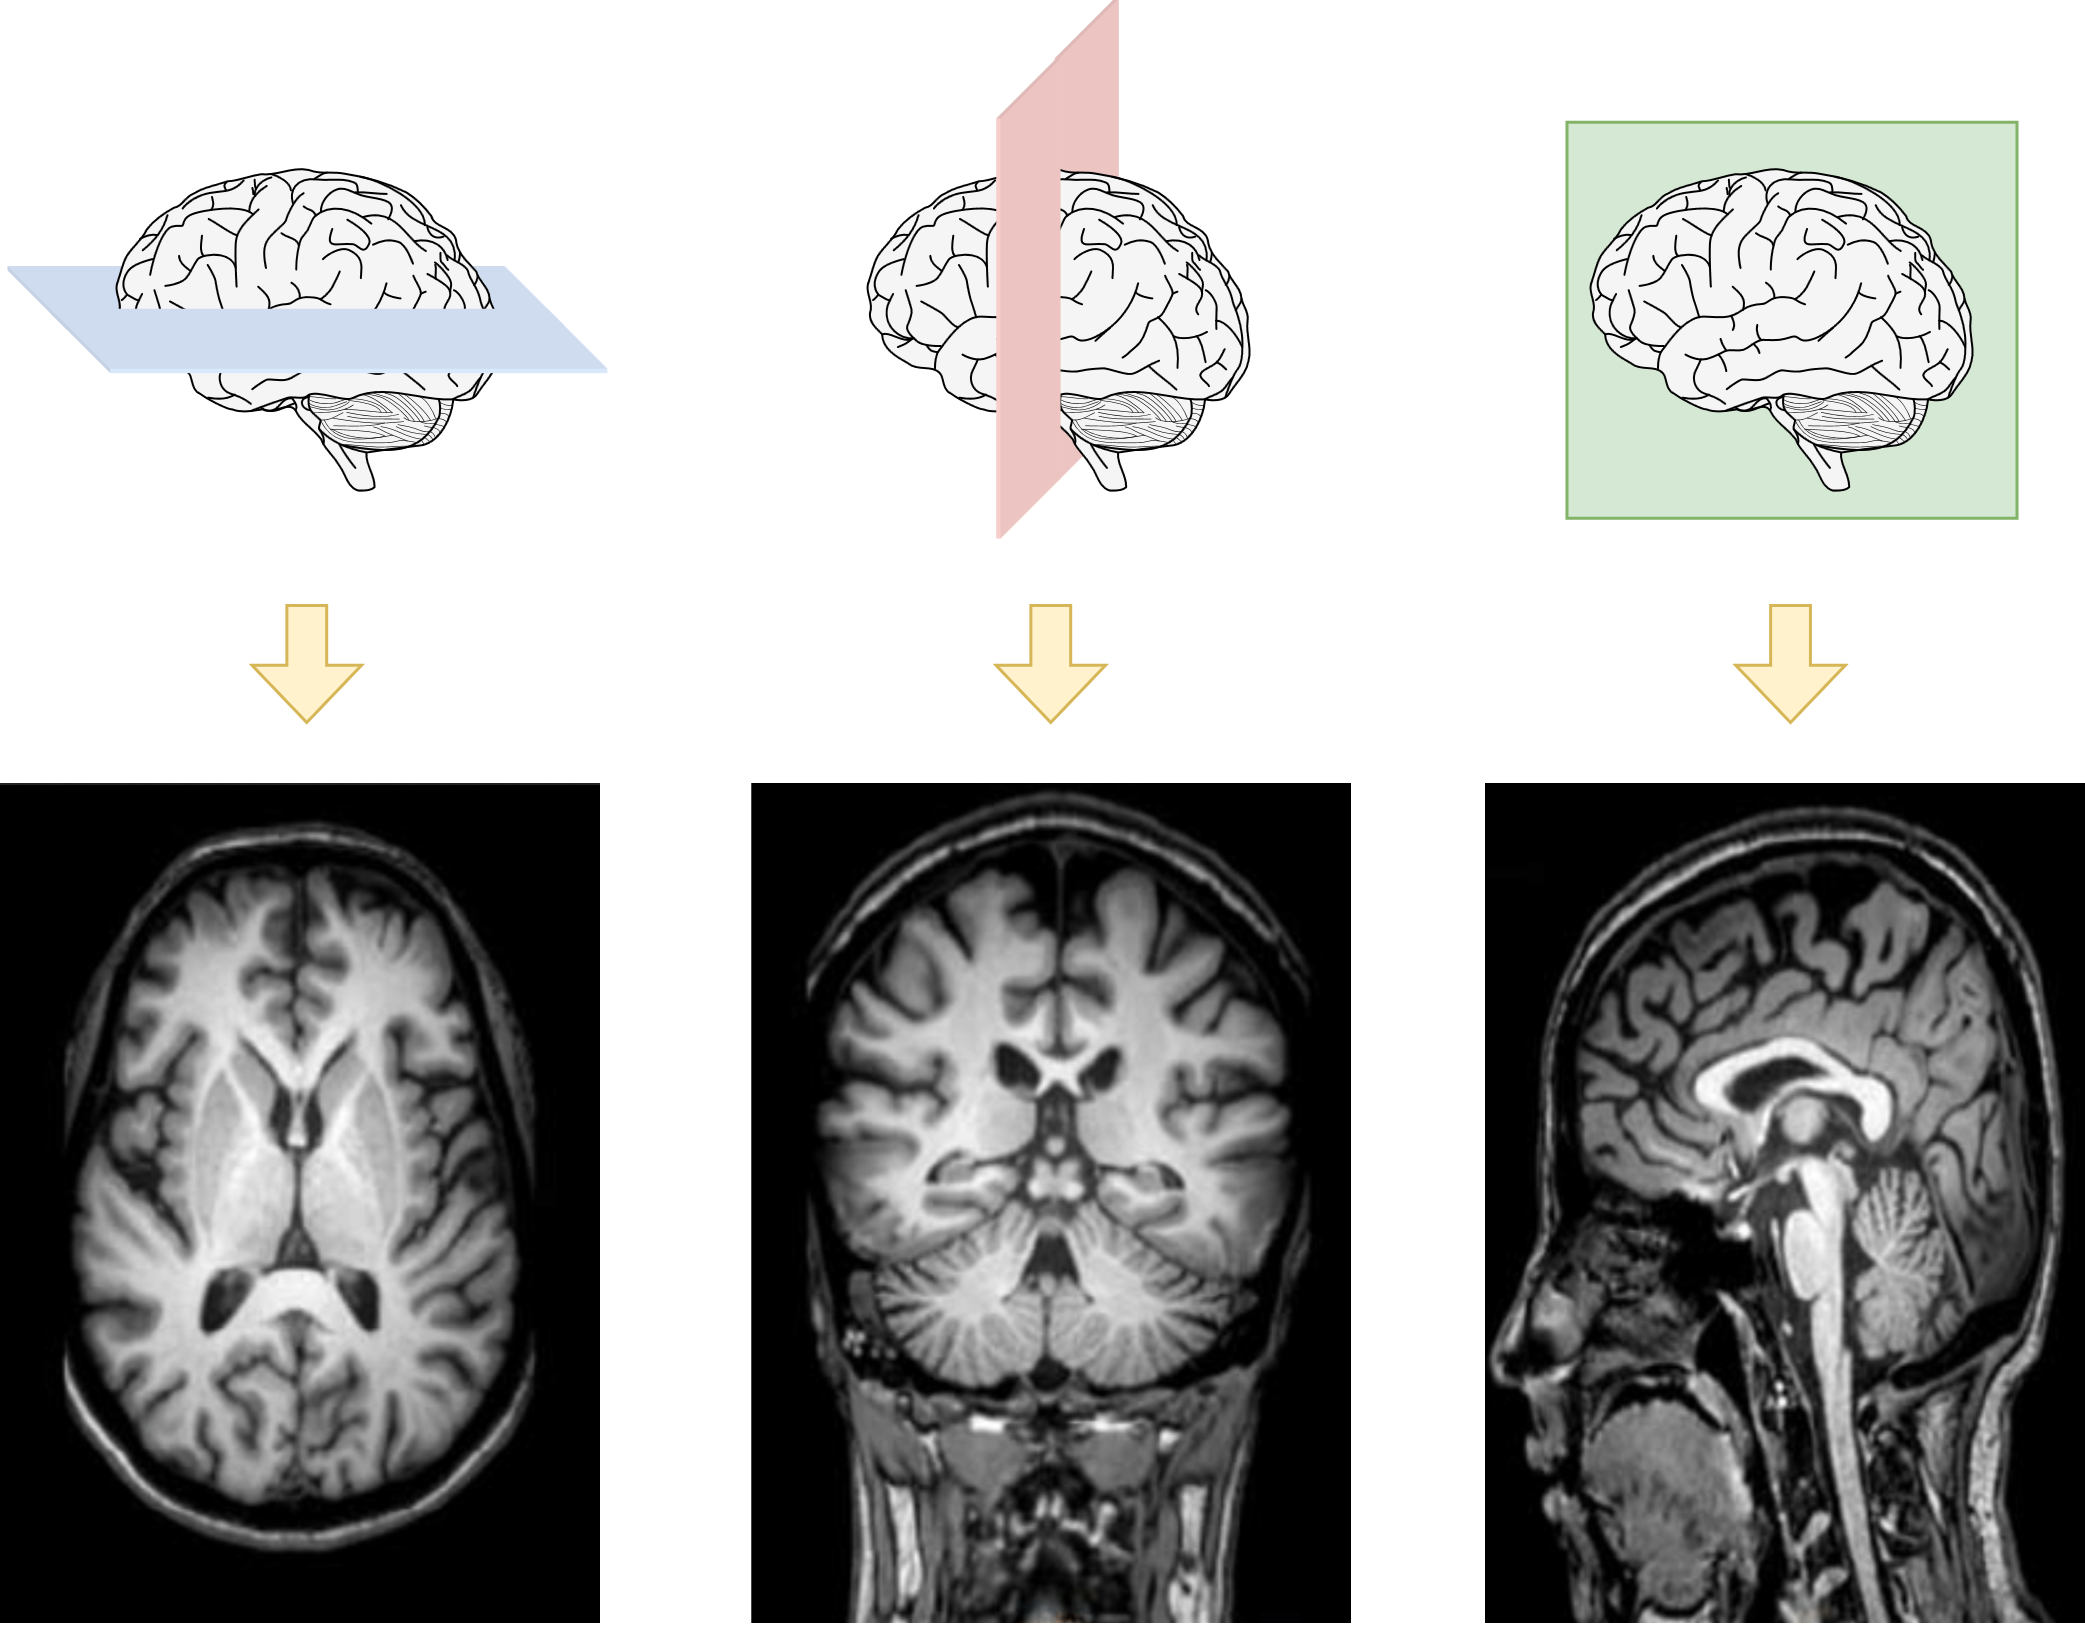
\includegraphics{3_1_acquisition_planes}
    \caption[Acquisiton Planes of an MRI Scan]{An MRI scan captures images of the brain from three different
    planes: axial, coronal, and sagittal. This figure shows the acquisition
    planes along with their corresponding generated images. The axial plane is
    depicted in blue, the coronal plane in red, and the sagittal plane in green.
    }
    \labfig{3_1}
\end{figure}
MR images are composed of digital image voxels, which are essentially 3D
volumes, in contrast to pixels that represent 2D squares. Each voxel in an MR
image contains a signal that represents all the MR-visible protons within that
specific volume. This setup allows for a three-dimensional representation of the
scanned area, providing depth that a two-dimensional pixel-based image cannot.

Higher magnetic field strengths in MR scanners enhance the quality of these
images. The stronger the magnetic field ($B_0$), the greater the level of detail
that can be achieved. This is because higher field strengths improve the
signal-to-noise ratio and the resolution of the images, allowing for better
differentiation of tissue types and more precise imaging of fine structures.
Consequently, MR scanners with higher field strengths are capable of producing
images with better clarity and more distinct separation of
signals\sidenote{For instance, MRI scanners commonly found in hospitals utilize
magnetic field strengths of either 1.5 Tesla or 3 Tesla.}

As mentioned earlier, each tissue type responds uniquely to the magnetic pulses
used in MR imaging. This differential response is precisely what the so called
T1 and T2 weighting exploit to enhance the visibility of various tissues within
the magnetic resonance images.
\begin{marginfigure}
    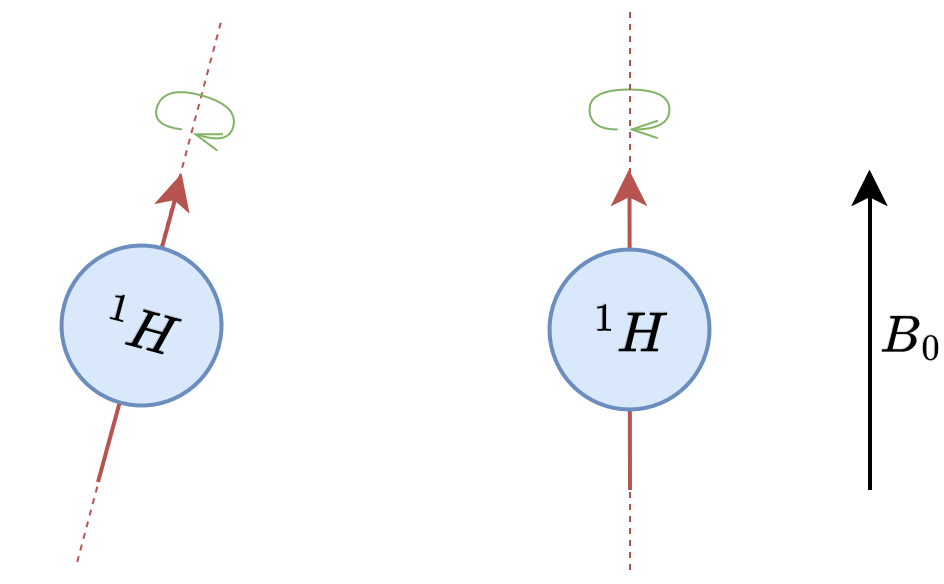
\includegraphics{3_2_spin_hydrogen}
    \caption[Spin of an Hydrogen Atom]{Hydrogen atoms spin along their axis.
    When a magnetic force is applied ($B_0$) their rotational axis is pulled
    towards the direction of the magnetic field.}
    \labfig{3_2}
\end{marginfigure}
T1-weighted imaging capitalizes on the \emph{longitudinal relaxation time}
($T_1$), which is the time it takes for protons to realign with the magnetic
field $B_0$ after the removal of the RF pulse. T1 times vary between different
types of tissue; for instance, fat has a shorter T1 time compared to water. In
T1-weighted images, tissues with shorter T1 relaxation times appear brighter.
Thus, these images are particularly effective for visualizing the anatomy of the
brain, distinguishing between grey and white matter, and identifying fatty
tissues, making them valuable for detailed anatomical studies.

T2-weighted imaging, on the other hand, emphasizes the \emph{transverse
relaxation time} ($T_2$), which is the time it takes for protons to lose phase
coherence among the directions perpendicular to the magnetic field, primarily
due to interactions with neighboring molecules. Tissues with longer T2 times,
such as fluids, appear brighter on T2-weighted images. This characteristic makes
T2-weighted imaging exceptionally useful for detecting fluid-filled areas, such
as edema, tumors, and inflammation in tissues.

The choice between T1 and T2 weighting depends on the diagnostic requirements;
T1 is preferred for detailed anatomical definition, while T2 is superior for
identifying fluid changes. This flexibility is a key strength of MRI technology,
allowing for tailored imaging that aligns closely with clinical and research
needs. In this work, the datasets used contained predominantly T1-weighted
images. 

\section{Voxel Based Morphometry}
Following the acquisition phase, MRI images can undergo analysis either
automatically (e.g., by a machine learning model) or manually. Nonetheless,
several inherent challenges may compromise the reliability of the data,
especially when comparing images across different individuals. Each individual's
brain presents distinct anatomical characteristics, including variations in
size, shape, and the distribution of tissues such as gray matter (GM), white
matter (WM), and cerebrospinal fluid (CSF). These discrepancies complicate
direct comparisons between scans because corresponding brain regions may not
align precisely across different individuals. This variability also impedes the
ability to draw comparisons or discern trends across populations or patient
groups\sidenote{Coincidently, a task that must be performed by Neural
Networks.}. Additionally, MRI scans are prone to various types of noise and
artifacts, which may originate from the scanner, environmental conditions, or
subject-related factors such as minor movements during scanning. These
extraneous signals can mask essential details critical for precise diagnosis or
effective research analysis.

To address these challenges, a pre-processing technique called Voxel-Based
Morphometry (VBM)~\sidecite{ashburner_vbm_2000} has been developed. VBM
standardizes and simplifies the process of comparing brain anatomy across
different individuals by focusing on measuring differences in the composition of
brain tissue, specifically the concentration and volume of gray and white
matter. The concept of VBM comprises three basic preprocessing steps: (1)
\emph{spatial normalization}, (2) \emph{tissue segmentation} , and (3)
\emph{spatial smoothing}, which are followed by the actual statistical analysis.

In the spatial normalization step, the MRI scans are matched together spatially
(registered) so that a location in one subject's MRI corresponds to the same
location in another subject's MRI. It is generally achieved by registering all
images from a study onto the same template image\sidenote[][*-4]{A common template
frequently used in the literature is the MNI (Montreal Neurological Institute)
template~\cite{evans_mni_1993}, which has also been utilized in this study.}
so that they are all in the same space. The template image could be one specific
MRI scan or could be created by averaging across a number of different MRI scans
that have been put in the same space.  After the template image has been
obtained, either linear or non linear transformations can be used to perform
this registration~\sidecite{kurth_vbm_2015}. 

The tissue segmentation process is the subsequent step, which involves
partitioning the MRI images into different tissue compartments such as white
matter (WM), gray matter (GM), and cerebrospinal fluid (CSF). As previously
discussed, in T1-weighted images (which are the focus of this thesis) the
longitudinal relaxation time ($T_1$) varies across different types of tissue.
Consequently, each tissue type displays a distinct level of brightness in the
images. This difference allows for the assignment of specific tissue types based
on their brightness levels. Essentially, this phase involves creating a map of
brightness values that correspond to different tissue types, enabling the
accurate identification of each tissue within the MRI images.
\begin{figure*}
    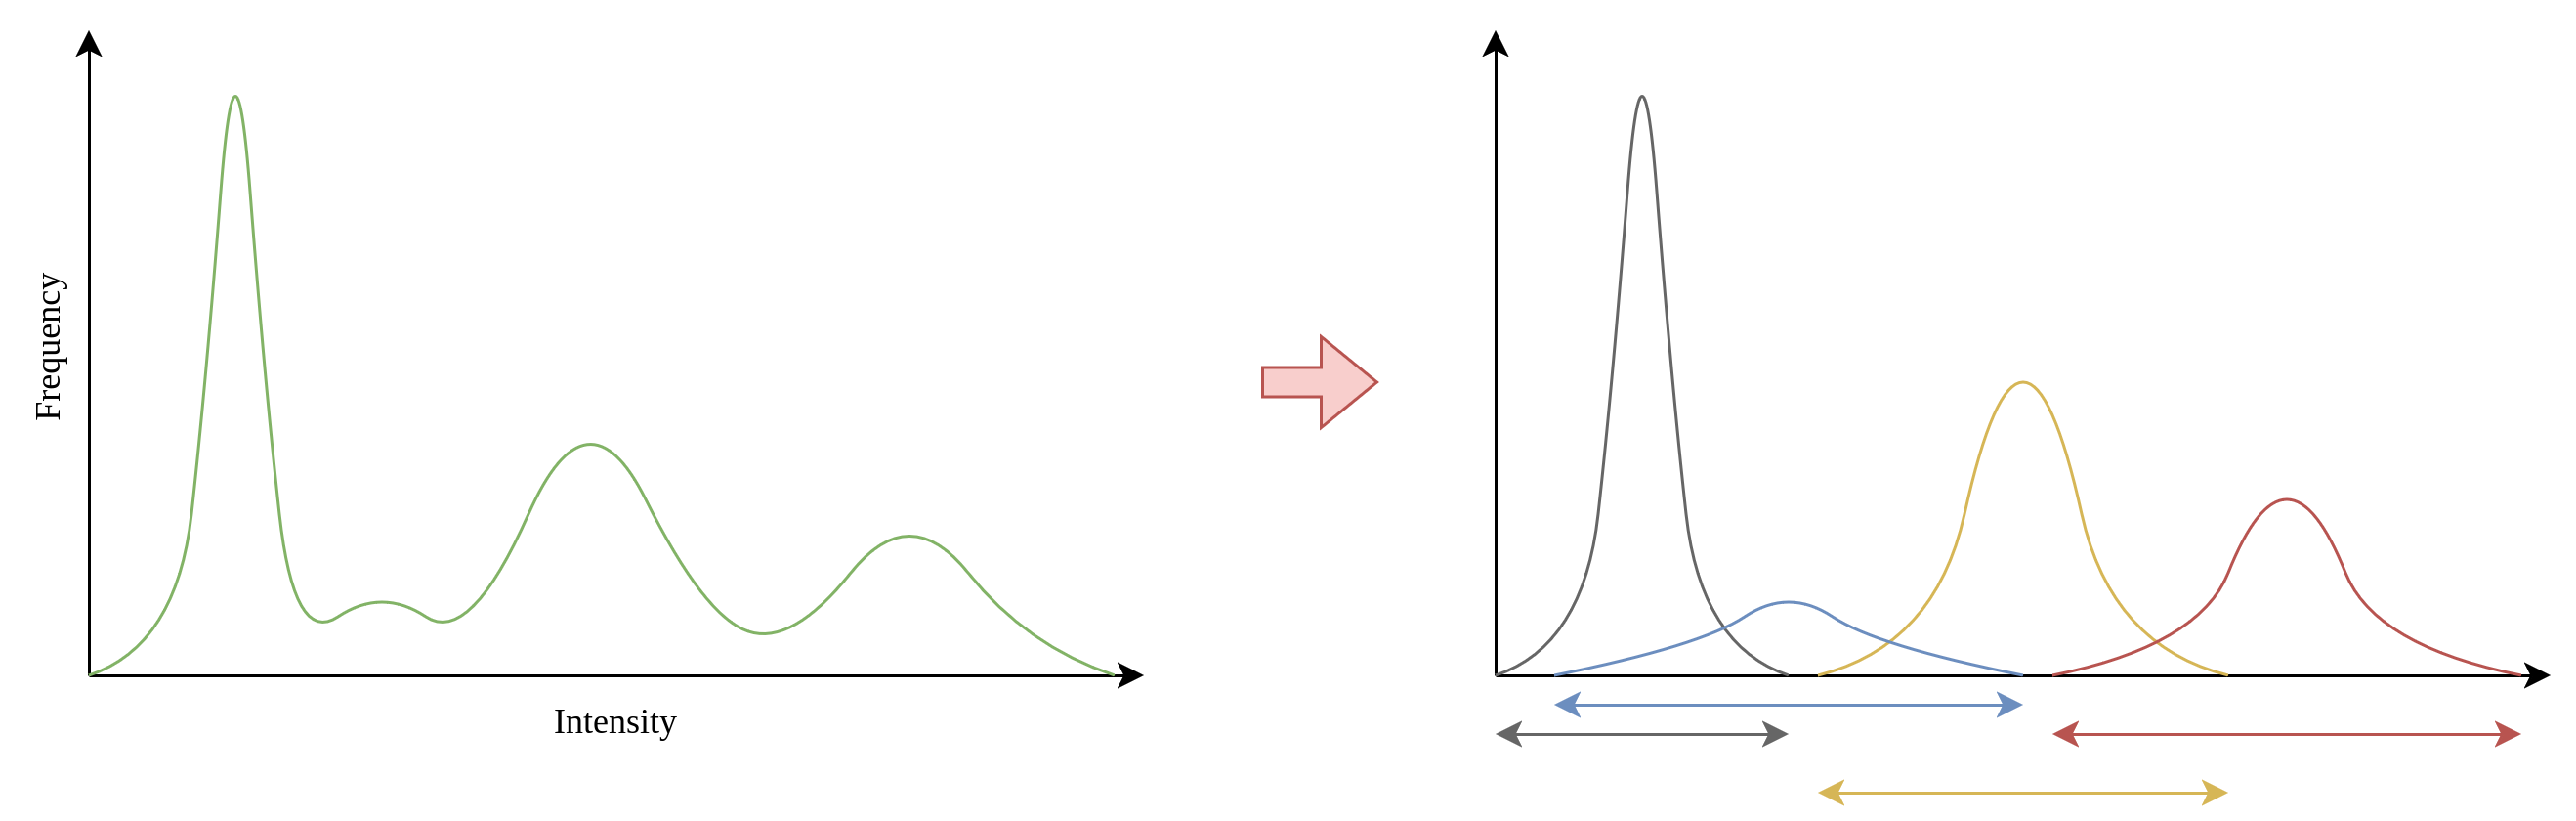
\includegraphics{3_3_segmentation_distribution}
    \caption[Segmentation (Values Distribution)]{On the left, an hypothetical
    distribution of intensity values of an MRI image. When this image undergoes
    tissue segmentation, the original distribution of intensity values is
    segmented into different distributions that represent a specific tissue
    class (right figure). For example, the gray one may represent background,
    the blue cerebrospinal fluid, the yellow white matter and the red grey
    matter. Note that in this case tissue-specific intensity distributions
    overlap. This is due to the fact that each voxel can contain more than one
    tissue.}
    \labfig{3_3}
\end{figure*}
To construct such a map, the distribution of intensity values within the MRI
images is divided into several smaller distributions, each representing a
specific tissue class. In practice, each voxel, commonly measuring $1mm$ isotropic, may contain multiple tissue types, causing overlaps
between the intensity distributions of different tissue classes. This overlap
can result in voxels being classified under more than one tissue category.

To address this challenge, tissue segmentation can be enhanced with the use of
additional probability maps that incorporate prior knowledge about the typical
locations of different tissues within the
brain~\sidecite{ashburner_segmentation_2005}. For each tissue type, a
probability map is used that indicates how likely a particular voxel is to
represent that tissue. This probabilistic approach helps to refine the decisions
made by the tissue classification algorithm, ensuring a more accurate
segmentation. Since the algorithm uses a probabilistic approach, the result is
an estimation of tissue composition for each voxel in the image.

The third and last step consist of a spatial smoothing, which consist on the
application of a convolution operation with a Gaussian filter\sidenote{A
Gaussian Filter is a kernel whose values are sampled from a Gaussian
distribution. In this case, they are sampled from a 3-dimensional Gaussian
distribution.}. The first is that smoothing can improve effectively the
signal-to-noise ratio by averaging the intensities of neighboring voxels. This
reduction in noise is essential because it helps to reveal the true anatomical
differences underlying the images, minimizing the impact of random fluctuations
that might otherwise be mistaken for significant variations.

Moreover, smoothing serves to increase the statistical power of the analyses
conducted in VBM. By making the data more normally distributed across voxels,
smoothing aligns with the statistical assumptions required for many of the
inferential techniques used in neuroimaging studies. This alignment is crucial
as it not only validates the use of parametric statistical tests but also
enhances the reliability of the findings by increasing the effective sample size
at each voxel. This approach provides a more robust basis for detecting
differences that are statistically significant rather than those arising from
the noise.
\begin{figure*}
    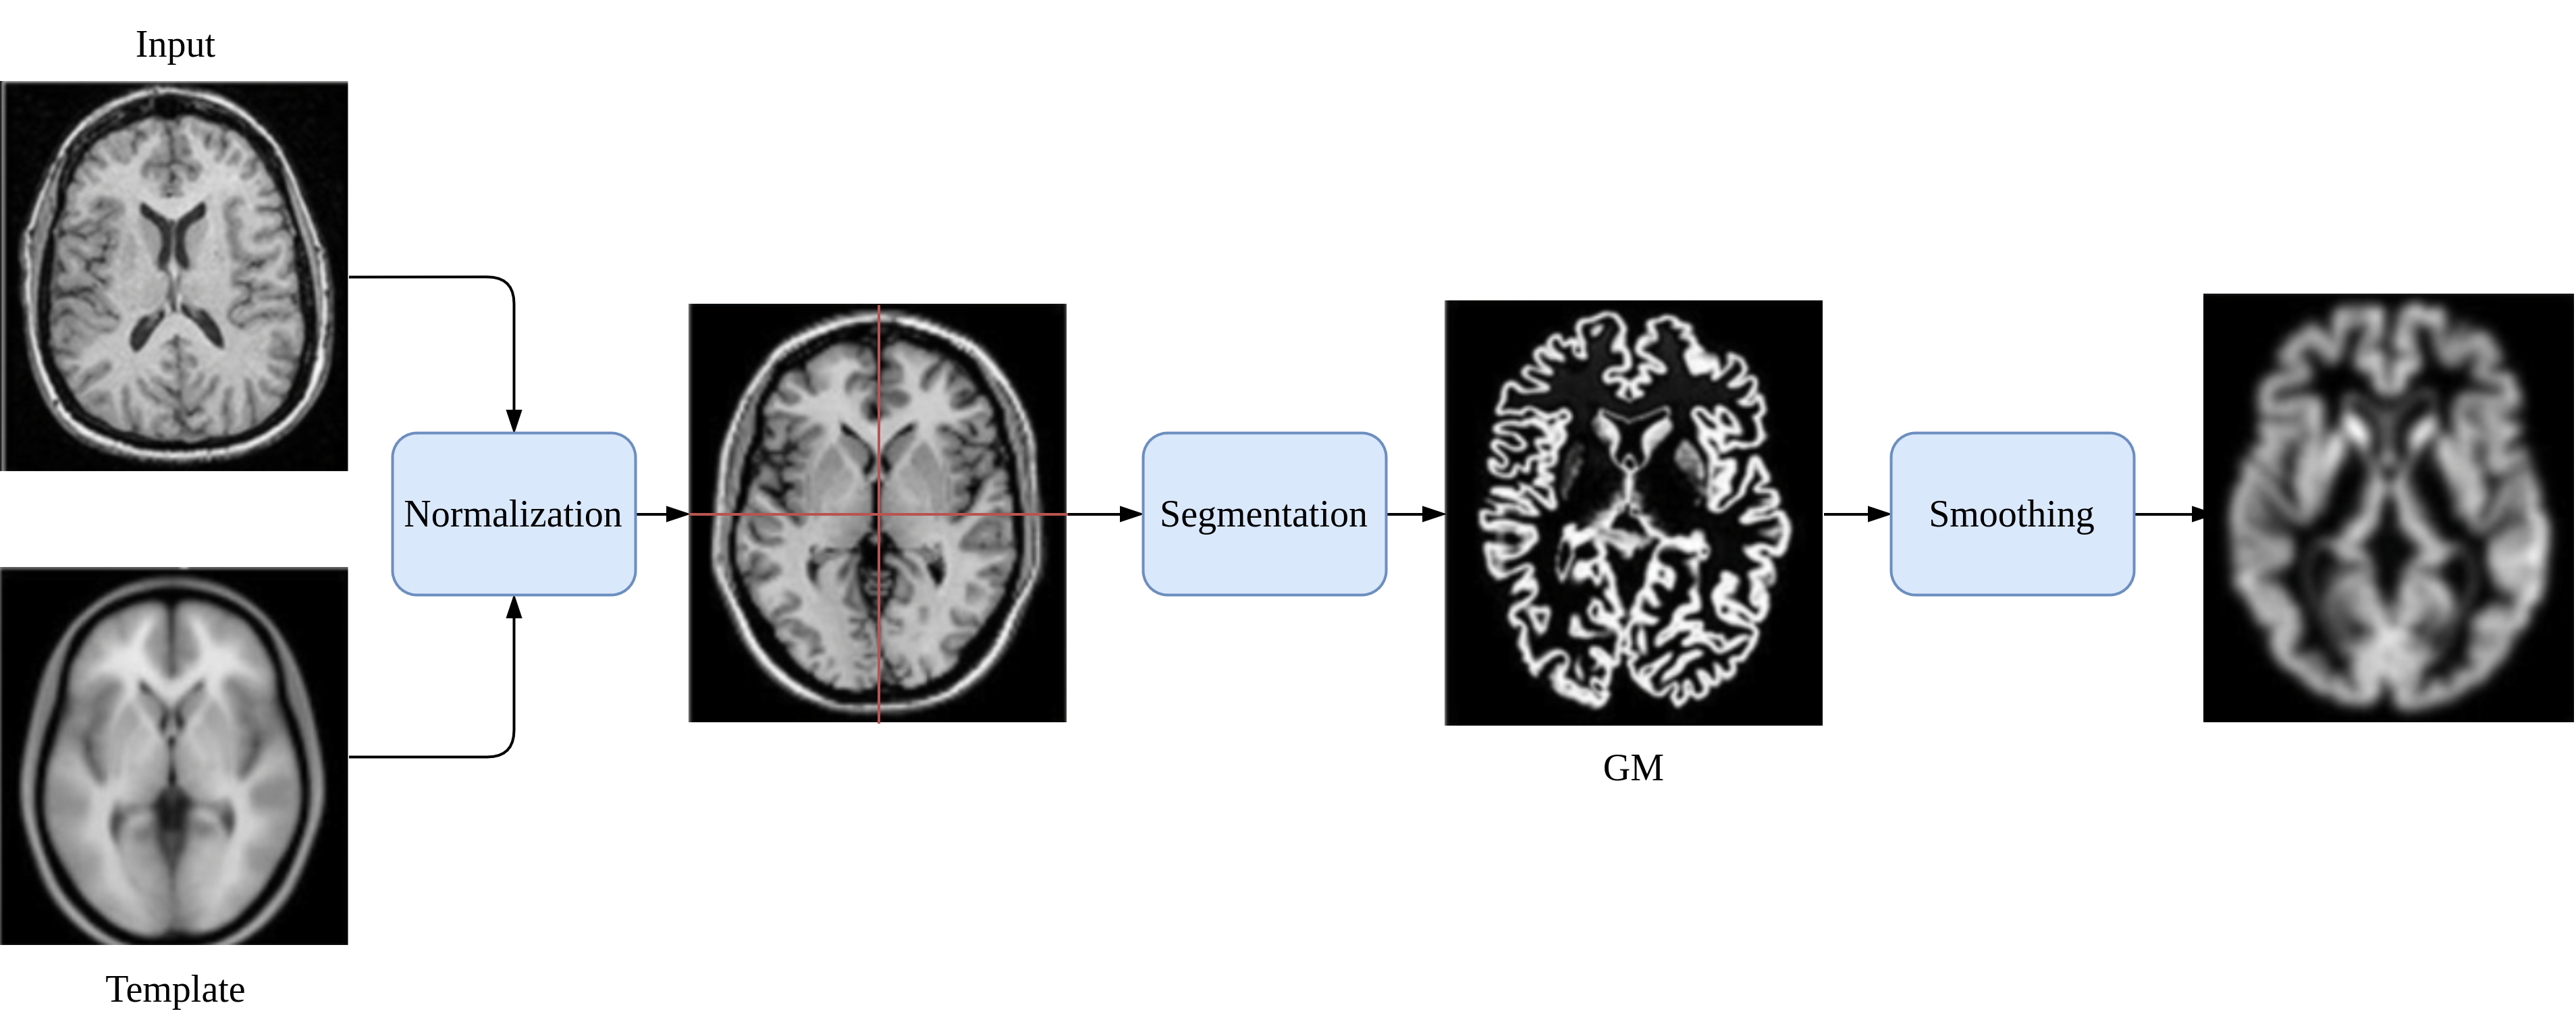
\includegraphics{3_4_vbm_steps}
    \caption[Voxel Based Morphometry Steps]{VBM processing is conducted in three
    steps. Initially, normalization is applied to all images using a standard
    template to ensure that they are aligned to the same frame of reference. The
    second step involves segmenting the normalized images into different tissue
    types, identifiable by their distinct intensity values. This segmentation
    results in the creation of separate volumes for each tissue type; for
    illustrative simplicity, only Gray Matter is depicted in this figure. The
    final step in the VBM process is the application of Gaussian smoothing to
    each of these segmented volumes.}
    \labfig{3_4}
\end{figure*}
Another key aspect of smoothing is its ability to account for minor registration
errors between subjects' images. Despite the application of the spatial
normalization step, slight misalignments can still occur due to the inherent
variability in brain anatomy among individuals. Smoothing helps to mitigate
these differences by blurring sharp edges and increasing the overlap of similar
anatomical structures across different scans. This adjustment is particularly
beneficial for ensuring accurate comparisons are made in studies comparing
groups of subjects, as it helps ensure that equivalent anatomical regions are
analyzed across all images.

Furthermore, smoothing is instrumental in matching the voxel-wise data to the
assumptions of Gaussian field theory, which underpins many of the statistical
methods used to draw inferences from neuroimaging data. This theory relies on
the smoothness of the data to make valid statistical claims about the presence
of significant brain regions. By applying a Gaussian filter, the data better
approximate a continuous Gaussian field, thus fulfilling the theoretical
prerequisites necessary for accurate \emph{p-value} calculation and hypothesis
testing.

Today there are various tools that perform VBM pre-processing, each with its own
choice for the implementations of the aforementioned steps. For the
pre-processing of MRI images used in this work, the
BrainPrep~\cite{grigis_brainprep_2022} software has been used, which is based on
two common pre-processing packages in neuroimaging CAT12~\cite{gaser_cat_2022}
and FreeSurfer~\cite{fischl_freesurfer_2012}.


\section{Brain Parcellations}
Brain parcellation is a method utilized in neuroimaging to divide the brain into
distinct regions based on anatomical landmarks, functional specialization, or
connectivity patterns. This technique is crucial for reducing the complexity of
the brain's architecture into manageable segments, thereby enabling more focused
and detailed analyses of its structure and function. Particularly in anatomical
MRI, parcellation proves invaluable for isolating specific areas of interest to
evaluate their individual contributions to overall brain anatomy.
\marginnote{The terms \emph{parcellation}, \emph{atlas}, and \emph{template} are
often used interchangeably in the literature.}The significance of brain
parcellation stems from its ability to enhance understanding of the
relationships and interactions among various parts of the brain. Segmenting the
brain into regions allows to effectively correlate specific structural changes
with cognitive functions or pathological states, facilitating deeper insights
into brain functionality and disorder.

Brain parcellations not only provide insights into the organizational principles
of the human brain but also offer significant practical benefits as biologically
informed strategies for data reduction. This process allows the information from
hundreds of thousands of voxels in MRI images to be compressed into a manageable
set of regions that reflect distinct
entities~\sidecite{eickhoff_parcellations_2018}. Such reduction is crucial,
particularly for neural network models, which can utilize this streamlined data
to predict behavioral or clinical phenotypes from brain imaging data. However,
for this aggregation to serve as a valid form of data compression, the
delineated parcels must represent a biologically meaningful patterning.

Over the past two decades, a variety of reliable brain parcellations have been
developed, each exhibiting specific strengths and weaknesses. These
parcellations have become essential tools for the analysis of neuroimaging
datasets. Depending on the type of data they utilize, and consequently the
acquisition method employed, these methods can be classified into three broad
categories~\sidecite{moghimi_parcellations_2021}:
\begin{itemize}
    \item Anatomical parcellations, which are constructed from T1-weighted MRI
    images.
    \item Functional parcellations, derived from from functional MRI (fMRI)
    images.
    \item Structural parcellations, based on diffusion-weighted-imaging
    data.
\end{itemize}
This thesis will specifically focus on anatomical parcellations. Within this
context, each defined region, known as a \emph{Region of Interest (ROI)}, is
assigned a specific label. As noted earlier, T1-weighted MRI images effectively
capture the anatomical structure of the brain. This includes the intricate
folding patterns of the cortical surface (its \emph{sulci} and
\emph{gyri}\sidenote[][*-4]{The cortical surface is the outer layer of neural
tissue of the brain. Sulci and gyri are the characteristic folds and ridges of
the brain, respectively.}) as well as sub-cortical structures\sidenote{Unlike
cortical structures, sub-cortical structures are anatomical features located
beneath the cortical surface.}.

A prevalent method for constructing anatomical parcellations involves using gyri
and sulci as markers to delineate the boundaries of regions of interest. The
brain displays prominent sulci that typically demarcate each functional area,
and by examining these major sulci, one can determine the boundaries of each
ROI. The process for identifying the landmarks used to define each ROI, along
with the number of ROIs, is encapsulated in a set of guidelines utilized by
neuroanatomy experts to manually label the MRI images. 

Given a specific set of guidelines, there are multiple methods for parcellating
new brain images. The approach discussed later in this thesis primarily involves
registering a new brain image to a template image that has already been manually
parcellated; this template is referred to as the \emph{reference atlas}.
Typically, a reference atlas is constructed from a collection of brain images
that have been manually segmented according to established guidelines. Once the
reference atlas is prepared, it facilitates the automatic parcellation of new
images.

Each atlas proposed in the literature adheres to a specific set of guidelines,
which results in variations in the number and delineation of Regions of Interest
(ROIs). This thesis will focus on two major atlases: the Desikan-Killiany
Atlas~\cite{desikan_automated_2006}, which has been predominantly utilized in
this research, and the Destrieux Atlas~\sidecite{destrieux_parcellation_2010}.
These atlases exemplify how differing guidelines can influence the definition
and segmentation of brain regions, impacting the analysis and interpretation of
neuroimaging data.

\subsection{Desikan-Killiany}
The Desikan-Killiany parcellation scheme divides the cortical area of the brain
into 34 regions of interest per hemisphere, resulting in a total of 68 ROIs for
the entire brain. To develop the Desikan atlas, the authors utilized a dataset
of 40 MRI scans that had been manually labeled by neuroanatomy experts. Various
sources of information were utilized to delineate the number of ROIs and their
anatomical boundaries, wich are discussed extensively in the original
publication~\cite{desikan_automated_2006} and are beyond the scope of this
discussion.

An automated algorithm, guided by the reference atlas, can
subsequently be applied to each new MRI scan to generate its corresponding
parcellation. In their foundational study, the authors compared a series of
automatically parcellated brains with manually parcellated counterparts. The
results demonstrated sufficient precision to affirm the method's anatomical
validity and reliability, indicating that this automated approach is both
effective and dependable for replicating established neuroanatomical
segmentations.

\begin{figure}
    \begin{subfigure}[h]{.5\linewidth}
        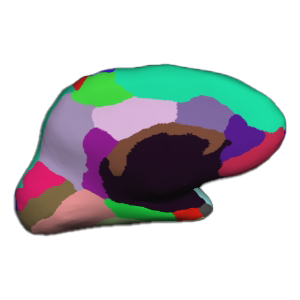
\includegraphics[width=1\linewidth]{3_5_a_desikan}
    \end{subfigure}%
    \begin{subfigure}[h]{0.5\linewidth}
        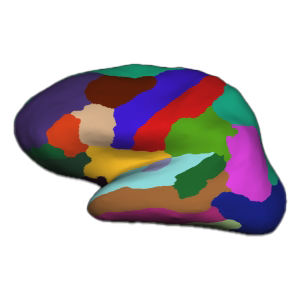
\includegraphics[width=1\linewidth]{3_5_b_desikan}
    \end{subfigure}
    \caption[Desikan Atlas]{Desikan Atlas. Each different color corresponds to a
    specific region of interest.}
\end{figure}

Each ROI within the Desikan scheme is characterized by a vector of different
anatomical measures, calculated over the corresponding volume represented by the
ROI. The selection of features depends on the image analysis software employed.
In this instance, the analysis software
utilized~\sidecite{fischl_freesurfer_2012} encompasses seven anatomical
measures. These measures provide a summary of various structural aspects of the
brain regions, which include:
\begin{itemize}
    \item \textbf{Average Cortical Thickness}: measures the average thickness of
    the cerebral cortex across the corresponding ROI.
    \item \textbf{Standard Deviation of Cortical Thickness}: measures the
    variability in terms of standard deviation of the cortical thickness within
    the ROI.
    \item \textbf{Gray Matter Volume}: quantifies the total volume of gray
    matter within the specified parcellated region.
    \item \textbf{Total Surface Area}: calculates the overall area of the
    cortical surface within each segmented region, relating to the extent of
    cortical folding.
    \item \textbf{Integrated Mean Curvature}: a differential geometry measure
    that computes the curvature of a surface by averaging the maximum and
    minimum curvatures registered across the ROI.
    \item \textbf{Gaussian Curvature}: similar to the Integrated Mean Curvature,
    but calculates the global curvature as the product of the minimum and
    maximum curvatures.
    \item \textbf{Intrinsic Curvature Index}: another measure to define global
    curvature, dependent on the distance between the highest and lowest
    curvatures of the surface.
\end{itemize}
Following this discussion, the Desikan parcellation process outputs a
corresponding matrix $\mathcal{D} \in \mathbb{R}^{68 \times 7}$, where each row
contains the discussed measures of a specific region of interest. This matrix
can be leveraged by deep learning models as additional data during the training
phase (as discussed in \refch{anatcl}) or as an alternative imaging format.

\subsection{Destrieux}
As previously noted, each anatomical atlas is distinctly shaped by the set of
guidelines that determine the number, position, and delineation of Regions of
Interest (ROIs). In the case of the Destrieux atlas, the guidelines were derived
from classical anatomical nomenclature as documented by
Duvernoy~\sidecite{duvernoy_brain_1999}. These rules were meticulously applied
to manually label each of twelve brains. The data from these manually
parcellated brains were subsequently utilized as a training set for a
statistical algorithm, which was employed to create the final Destrieux
reference atlas. The resulting atlas comprises 74 regions of interest for each
brain hemisphere, culminating in a total of 148 ROIs. Despite these differences
from other atlases, the Destrieux atlas retains the same anatomical measures for
each ROI. Consequently, a Destrieux atlas for a particular brain can be
systematically represented in a matrix format, $\mathcal{D} \in \mathbb{R}^{148
\times 7}$, where each row corresponds to an ROI and each column to one of seven
the anatomical measures.
\begin{figure}[h]
    \begin{subfigure}[h]{.5\linewidth}
        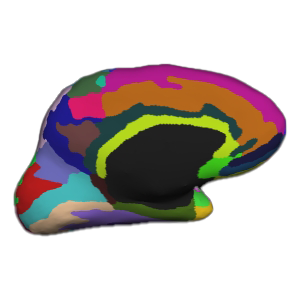
\includegraphics[width=1\linewidth]{3_6_a_destrieux}
    \end{subfigure}%
    \begin{subfigure}[h]{0.5\linewidth}
        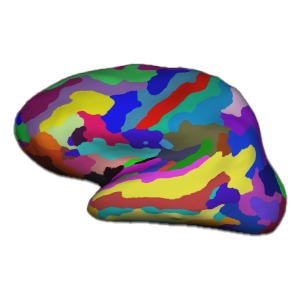
\includegraphics[width=1\linewidth]{3_6_b_destrieux}
    \end{subfigure}
    \caption[Destrieux Atlas]{Destrieux Atlas. Each different color corresponds
    to a specific region of interest.}
\end{figure}